\pageIconOpt
\ainfoX{\CTNT}{The 24\thsup International Conference on Verification, Model Checking, and Abstract Interpretation (VMCAI), 2023}
{\noindent Software artifact: \href{https://zenodo.org/records/7080145}{10.5281/zenodo.7080145}
\newline\noindent Citation:~\cite{aubert202213}
\newline\newline\textit{Reproduced with permission from Springer Nature.}}
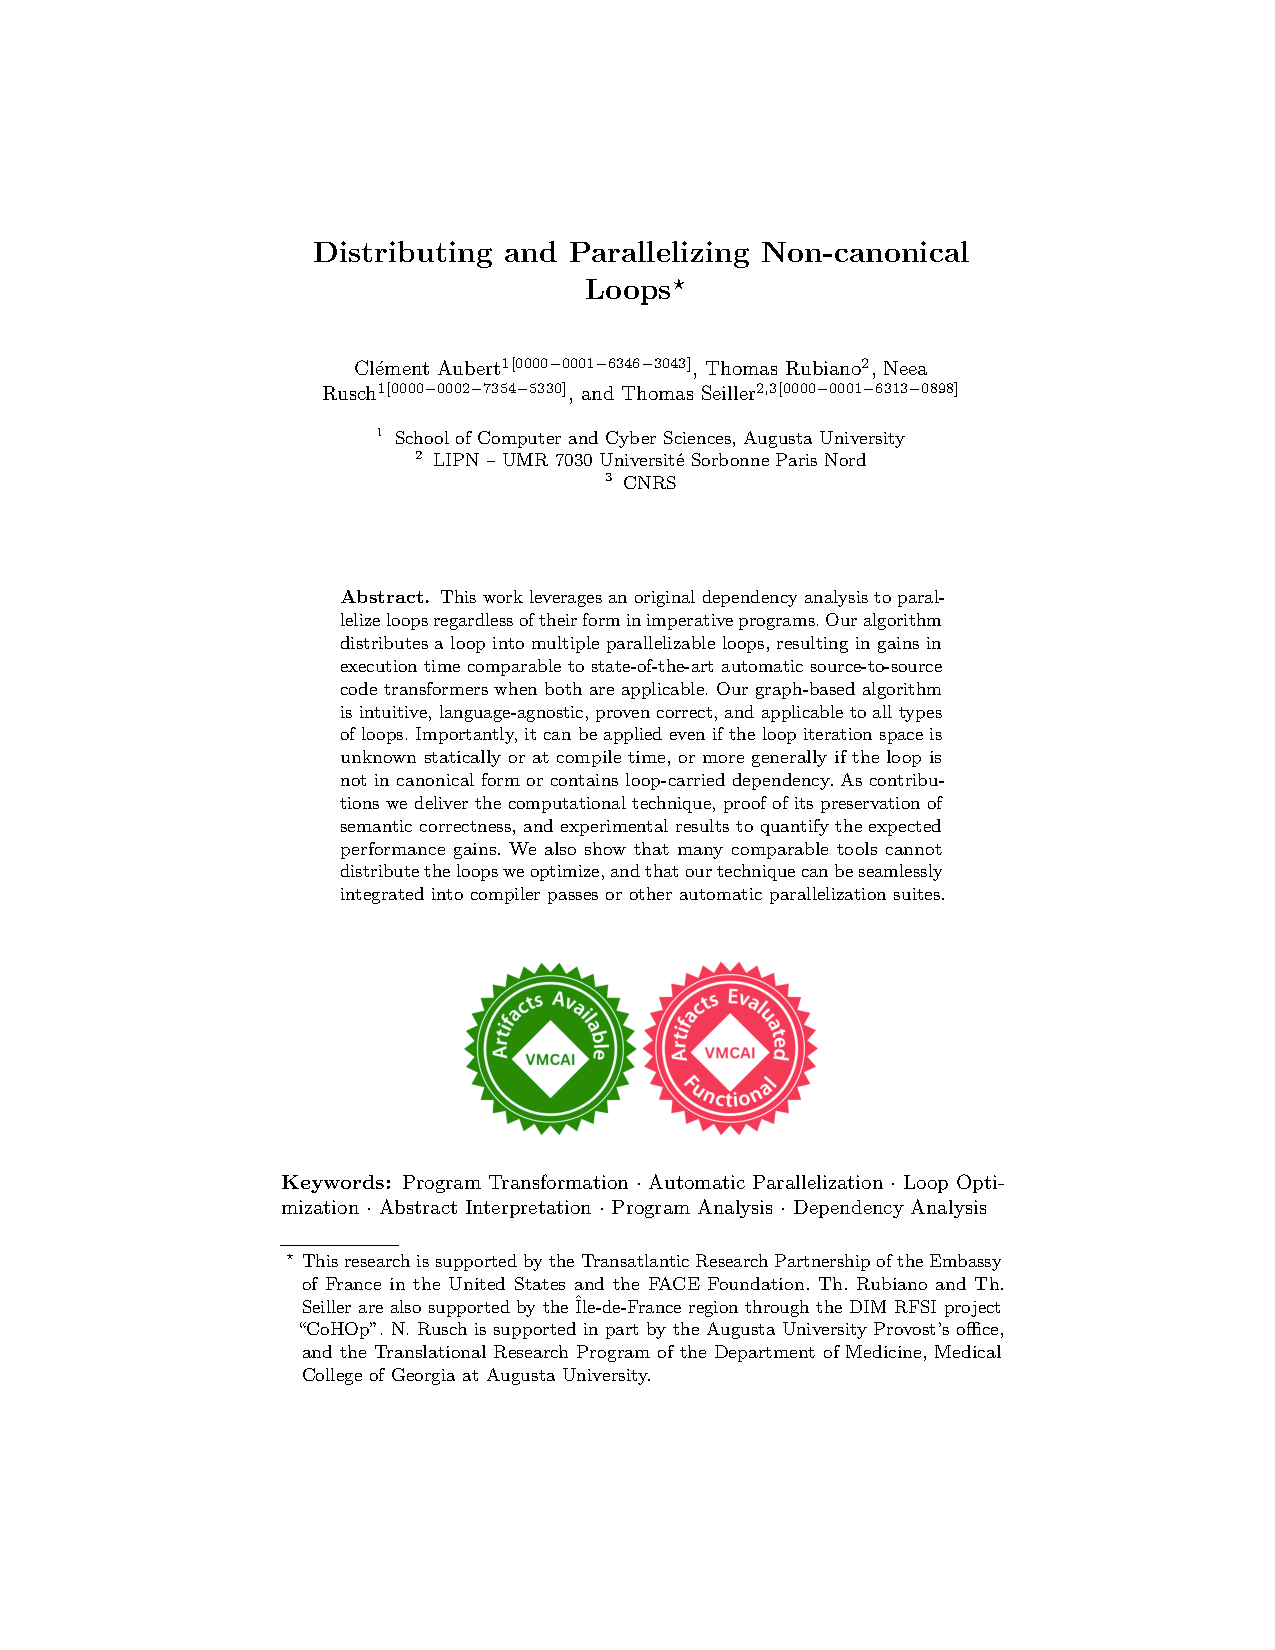
\includepdf[pages={1-},addtotoc={
    2,subsection,2,{Original Approaches to Automatic Parallelization},sec:vmcai-intro,
    4,subsection,2,{Background: Language and Dependency Analysis},sec:vmcai-background,
    11,subsection,2,{Loop Fission Algorithm},sec:fission-algo,
    14,subsection,2,{Limitations of Existing Alternative Approaches},sec:vmcai-limitations,
    16,subsection,2,{Evaluation},sec:vmcai-eval,
    21,subsection,2,{Conclusion},sec:vmcai-conc},
    addtolist={
        5,figure,{Simple imperative while language},fig-grammar,
        6,table,{Definition of Out, In and Occ for commands},table:def-out-in-occ,
        8,figure,{Statement examples, sets, and representations of their dependencies},fig:dependences,
        9,figure,Data-Flow Graph of composition,fig:composition,
        13,figure,Distributing a more complex while loop,fig:exampe-complex,
        16,table,Parallelization tools feature support comparison,tab:comparison,
        17,figure,Code transformation example,fig:code-example,
        19,figure,Speedup of selected benchmarks,fig:while,
        20,table,Speedup comparison between parallel benchmarks,tab:speedup,
        20,table,Descriptions of evaluated parallel benchmarks,tab:benchmarks},
    pagecommand={\thispagestyle{empty}%
    \addtoindex{Clava}{15}
    \addtoindex{Clava}{16}
    \addtoindex{Clava}{19}
    \addtoindex{Cetus}{15}
    \addtoindex{Cetus}{16}
    \addtoindex{MiBench}{17}
    \addtoindex{MiBench}{20}
    \addtoindex{NAS Parallel Benchmarks}{17}
    \addtoindex{NAS Parallel Benchmarks}{20}
    \addtoindex{OpenMP}{14}
    \addtoindex{OpenMP}{15}
    \addtoindex{OpenMP}{16}
    \addtoindex{OpenMP}{18}
    \addtoindex{OpenMP}{19}
    \addtoindex{OpenMP}{20}
    \addtoindex{OpenMP}{2}
    \addtoindex{OpenMP}{3}
    \addtoindex{OpenMP}{4}
    \addtoindex{matrix!empty}{7}
    \addtoindex{Par4All}{15}
    \addtoindex{Par4All}{16}
    \addtoindex{Pluto}{15}
    \addtoindex{Pluto}{16}
    \addtoindex{Polybench/C}{16}
    \addtoindex{Polybench/C}{17}
    \addtoindex{Polybench/C}{18}
    \addtoindex{ROSE}{14}
    \addtoindex{ROSE}{15}
    \addtoindex{ROSE}{16}
    \addtoindex{ROSE}{17}
    \addtoindex{ROSE}{18}
    \addtoindex{ROSE}{19}
    \addtoindex{ROSE}{20}
    \addtoindex{TRACO}{15}
    \addtoindex{TRACO}{16}
    \addtoindex{compilation!parallelizing}{15}
    \addtoindex{compilation!parallelizing}{16}
    \addtoindex{compilation!parallelizing}{17}
    \addtoindex{compilation!parallelizing}{19}
    \addtoindex{compilation!parallelizing}{3}
    \addtoindex{compilation!source-to-source}{15}
    \addtoindex{compilation!source-to-source}{1}
    \addtoindex{compilation!source-to-source}{3}
    \addtoindex{dependency analysis}{14}
    \addtoindex{dependency analysis}{21}
    \addtoindex{dependency analysis}{2}
    \addtoindex{dependency analysis}{4}
    \addtoindex{dependency analysis}{6}
    \addtoindex{graph!bi-partite}{7}
    \addtoindex{graph!condensation}{11}
    \addtoindex{graph!condensation}{12}
    \addtoindex{graph!condensation}{13}
    \addtoindex{graph!covering}{11}
    \addtoindex{graph!covering}{12}
    \addtoindex{graph!covering}{13}
    \addtoindex{graph!covering}{14}
    \addtoindex{graph!data-flow}{6}
    \addtoindex{graph!data-flow}{7}
    \addtoindex{graph!dependence}{11}
    \addtoindex{graph!dependence}{14}
    \addtoindex{graph!dependence}{15}
    \addtoindex{saturated covering}{12}
    \addtoindex{saturated covering}{13}
    \addtoindex{Intel's C++ compiler}{15}
    \addtoindex{Intel's C++ compiler}{16}
    \addtoindex{loop form!canonical}{15}
    \addtoindex{loop form!canonical}{16}
    \addtoindex{loop form!canonical}{17}
    \addtoindex{loop form!canonical}{2}
    \addtoindex{loop form!canonical}{4}
    \addtoindex{loop form!non-canonical}{21}
    \addtoindex{loop form!non-canonical}{2}
    \addtoindex{loop transformation!distribution}{2}
    \addtoindex{loop transformation!fission}{11}
    \addtoindex{loop transformation!fission}{12}
    \addtoindex{loop transformation!fission}{14}
    \addtoindex{loop transformation!fission}{15}
    \addtoindex{loop transformation!fission}{16}
    \addtoindex{loop transformation!fission}{17}
    \addtoindex{loop transformation!fission}{18}
    \addtoindex{loop transformation!fission}{19}
    \addtoindex{loop transformation!fission}{20}
    \addtoindex{loop transformation!fission}{2}
    \addtoindex{loop transformation!fission}{3}
    \addtoindex{loop transformation!fission}{4}
    \addtoindex{loop transformation!fission}{6}
    \addtoindex{loop transformation!tiling}{4}
    \addtoindex{loop transformation!fusion}{21}
    \addtoindex{loop transformation!unrolling}{21}
    \addtoindex{loop transformation!unrolling}{3}
    \addtoindex{loop-carried dependency}{15}
    \addtoindex{loop-level parallelism}{2}
    \addtoindex{automatic parallelization}{15}
    \addtoindex{automatic parallelization}{16}
    \addtoindex{automatic parallelization}{19}
    \addtoindex{automatic parallelization}{20}
    \addtoindex{automatic parallelization}{3}
    \addtoindex{automatic parallelization}{4}
    \addtoindex{parallelization potential}{3}
    \addtoindex{polyhedral optimization}{4}
    \addtoindex{state explosion}{3}
    \addtosymbols{corro}{9}
    \addtosymbols{corr}{10}
    \addtosymbols{corr}{8}
    \addtosymbols{corr}{9}
    \addtosymbols{dfg}{10}
    \addtosymbols{dfg}{11}
    \addtosymbols{dfg}{7}
    \addtosymbols{dfg}{8}
    \addtosymbols{et}{9}
    \addtosymbols{graphw}{11}
    \addtosymbols{graphw}{12}
    \addtosymbols{graph}{12}
    \addtosymbols{infty2}{10}
    \addtosymbols{infty2}{11}
    \addtosymbols{infty2}{7}
    \addtosymbols{infty2}{8}
    \addtosymbols{infty2}{9}
    \addtosymbols{looppw}{12}
    \addtosymbols{looppw}{13}
    \addtosymbols{looppw}{14}
    \addtosymbols{loopw}{10}
    \addtosymbols{loopw}{11}
    \addtosymbols{loopw}{12}
    \addtosymbols{loopw}{13}
    \addtosymbols{loopw}{14}
    \addtosymbols{mdfg}{10}
    \addtosymbols{mdfg}{11}
    \addtosymbols{mdfg}{13}
    \addtosymbols{mdfg}{7}
    \addtosymbols{mdfg}{8}
    \addtosymbols{mdfg}{9}
    \addtosymbols{occ}{10}
    \addtosymbols{occ}{6}
    \addtosymbols{occ}{7}
    \addtosymbols{occ}{9}
    \addtosymbols{one}{10}
    \addtosymbols{one}{7}
    \addtosymbols{one}{8}
    \addtosymbols{one}{9}
    \addtosymbols{vin}{11}
    \addtosymbols{vin}{6}
    \addtosymbols{vin}{7}
    \addtosymbols{vin}{8}
    \addtosymbols{vout}{10}
    \addtosymbols{vout}{11}
    \addtosymbols{vout}{6}
    \addtosymbols{vout}{7}
    \addtosymbols{vout}{8}
    \addtosymbols{vout}{9}
    \addtosymbols{zero2}{10}
    \addtosymbols{zero2}{7}
    \addtosymbols{zero2}{8}
    \addtosymbols{zero2}{9}
    }]{pdf/pubs_vmcai.2023.pdf}